\documentclass[9pt]{beamer}

\usepackage[utf8x]{inputenc}
\usepackage[english]{babel}
\usepackage{amsmath, amsfonts, amssymb}
\usepackage{color}
\usepackage{xcolor}
\usepackage{tikz}
\usetikzlibrary{positioning,shapes,shadows,arrows,snakes}
\usepackage{listliketab}
\usepackage{shuffle}
\usepackage{xargs}
\usepackage{multirow}
\usepackage{pgfplots}
\usepackage{csquotes}
\usepackage{verbatim}

\definecolor{BlueGreen}{cmyk}{0.85,0,0.33,0}
\definecolor{RawSienna}{cmyk}{0,0.72,1,0.45}
\definecolor{gold}{rgb}{1.,0.84,0.}
\definecolor{dgreen}{rgb}{0.,0.6,0.}

\definecolor{Noir}{RGB}{0,0,0}
\definecolor{Rouge}{RGB}{205,35,38}
\definecolor{Bleu}{RGB}{2,60,195}
\definecolor{Bleu1}{RGB}{121,176,197}
\definecolor{Vert}{RGB}{23,103,1}
\definecolor{VertOlive}{RGB}{112,141,35}
\definecolor{Orange}{RGB}{255,113,15}
\definecolor{RoseBonbon}{RGB}{249,66,158}
\definecolor{Marron}{RGB}{193,88,50}

\definecolor{mygreen}{RGB}{23,103,1}

\newcommand{\red}[1]{\textcolor{red}{#1}}
\newcommand{\blue}[1]{\textcolor{blue}{#1}}
\newcommand{\green}[1]{\textcolor{mygreen}{#1}}
\newcommand{\bluealert}[2]{\textcolor<#1>{blue}{#2}}

\tikzstyle{alert} = [color=red, line width = 1.5]
\tikzstyle{bluealert} = [color=blue, line width =1.5]
\tikzstyle{big} = [line width = 1.5]
\tikzstyle{Point} = [fill, radius=0.08]
\tikzstyle{RedPoint} = [fill, radius=0.09, color = red]


\tikzstyle{Red} = [color = red]
\tikzstyle{Blue} = [color = blue]
\tikzstyle{Green} = [color = Vert]
\tikzstyle{Gray} = [color = gray]

\definecolor{violet}{rgb}{.5,.1,.9}


\usetheme{Boadilla}
\title{Adversarial examples in deep learning}
\author{G. Châtel}
\date{06/07/2017}

\begin{document}

%%%%%%%%%%%%%%%%%%%%%%%%%%%%%%%%%%%%%%%%%%%%%%%%%%%%%%%%%%%%%%%%%%%%%%
\begin{frame}

  \maketitle

\end{frame}
%%%%%%%%%%%%%%%%%%%%%%%%%%%%%%%%%%%%%%%%%%%%%%%%%%%%%%%%%%%%%%%%%%%%%%

%%%%%%%%%%%%%%%%%%%%%%%%%%%%%%%%%%%%%%%%%%%%%%%%%%%%%%%%%%%%%%%%%%%%%%
\begin{frame}

  \tableofcontents

\end{frame}
%%%%%%%%%%%%%%%%%%%%%%%%%%%%%%%%%%%%%%%%%%%%%%%%%%%%%%%%%%%%%%%%%%%%%%

\section{Introduction}

%%%%%%%%%%%%%%%%%%%%%%%%%%%%%%%%%%%%%%%%%%%%%%%%%%%%%%%%%%%%%%%%%%%%%%
\begin{frame}
  \frametitle{Basic notions}

  An adversarial example is a sample of input data which has been
  modified very slightly in a way that is intended to cause a machine
  learning classifier to misclassify it.
\end{frame}
%%%%%%%%%%%%%%%%%%%%%%%%%%%%%%%%%%%%%%%%%%%%%%%%%%%%%%%%%%%%%%%%%%%%%%

%%%%%%%%%%%%%%%%%%%%%%%%%%%%%%%%%%%%%%%%%%%%%%%%%%%%%%%%%%%%%%%%%%%%%%
\begin{frame}

\end{frame}
%%%%%%%%%%%%%%%%%%%%%%%%%%%%%%%%%%%%%%%%%%%%%%%%%%%%%%%%%%%%%%%%%%%%%%

%%%%%%%%%%%%%%%%%%%%%%%%%%%%%%%%%%%%%%%%%%%%%%%%%%%%%%%%%%%%%%%%%%%%%%
\begin{frame}
  \frametitle{Gradient descent}

  \begin{center}
    \scalebox{0.5}{
      \begin{tikzpicture}[xscale = 3.5, yscale=3.5]
  \foreach \Point in { (0.418313, 0.604578), (0.196620, 0.549155),
    (0.734198, 0.683549), (0.767944, 0.691986), (0.212015, 0.553004),
    (0.866296, 0.716574), (0.741085, 0.685271), (0.091187, 0.522797),
    (0.957083, 0.739271), (0.400345, 0.600086), (0.110229, 0.527557),
    (0.628896, 0.657224), (0.079816, 0.519954), (0.585337, 0.646334),
    (0.240140, 0.560035), (0.712331, 0.678083), (0.810917, 0.702729),
    (0.262672, 0.565668), (0.690066, 0.672516), (0.871858, 0.717964),
    (0.444774, 0.611194), (0.021740, 0.505435), (0.308306, 0.577077),
    (0.055931, 0.513983), (0.343537, 0.585884), (0.007552, 0.501888),
    (0.614842, 0.653711), (0.343214, 0.585804), (0.627016, 0.656754),
    (0.951821, 0.737955) }{ 
    \node at \Point {
      \textbullet
    }; 
  }

  \draw[->] (0, 0) -- (1.2, 0) node[right] {$x$};
  \draw[->] (0, 0) -- (0, 1.2) node[above] {$y$};
  \draw (1, 0.25pt) -- (1, -0.5pt) node[anchor = north]{1};
  \draw (0.25pt, 1) -- (-0.5pt, 1) node[anchor = east]{1};
\end{tikzpicture}

    }
  \end{center}

  We have a set of points that we want to approximate with a line.

  \[
  y = ax + b
  \]

  \pause

  First we choose a \textcolor{blue}{loss} that measures how good our
  predictions are.

  \[
  l(x, y, a, b) = (y - (a x + b))^{2}
  \]

  \pause

  We compute how the loss is affected by small changes of $a$ and
  $b$:

  \[
  \frac{dl}{da} = 2 x (ax + b - y) \qquad \qquad \frac{dl}{db} = 2 (ax + b - y)
  \]

  And we update $a$ and $b$ iteratively until we reach a satisfying
  result (the average loss is low enough).

%  a = -0.08 \quad b = 0.68
\end{frame}
%%%%%%%%%%%%%%%%%%%%%%%%%%%%%%%%%%%%%%%%%%%%%%%%%%%%%%%%%%%%%%%%%%%%%%

%%%%%%%%%%%%%%%%%%%%%%%%%%%%%%%%%%%%%%%%%%%%%%%%%%%%%%%%%%%%%%%%%%%%%%
\begin{frame}
  \frametitle{Gradient descent}

  \begin{center}
    \scalebox{0.5}{
      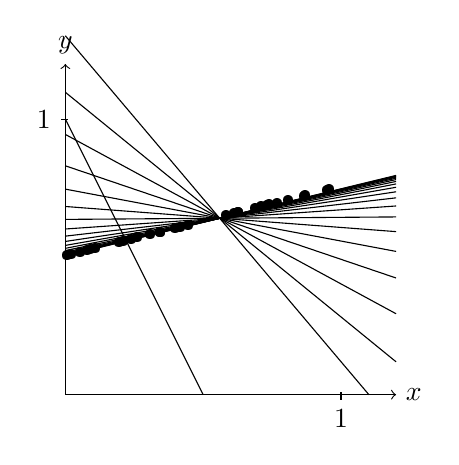
\begin{tikzpicture}[xscale = 3.5, yscale=3.5]
  \foreach \Point in { (0.418313, 0.604578), (0.196620, 0.549155),
    (0.734198, 0.683549), (0.767944, 0.691986), (0.212015, 0.553004),
    (0.866296, 0.716574), (0.741085, 0.685271), (0.091187, 0.522797),
    (0.957083, 0.739271), (0.400345, 0.600086), (0.110229, 0.527557),
    (0.628896, 0.657224), (0.079816, 0.519954), (0.585337, 0.646334),
    (0.240140, 0.560035), (0.712331, 0.678083), (0.810917, 0.702729),
    (0.262672, 0.565668), (0.690066, 0.672516), (0.871858, 0.717964),
    (0.444774, 0.611194), (0.021740, 0.505435), (0.308306, 0.577077),
    (0.055931, 0.513983), (0.343537, 0.585884), (0.007552, 0.501888),
    (0.614842, 0.653711), (0.343214, 0.585804), (0.627016, 0.656754),
    (0.951821, 0.737955) }{ 
    \node at \Point {
      \textbullet
    }; 
  }

  \draw[->] (0, 0) -- (1.2, 0) node[right] {$x$};
  \draw[->] (0, 0) -- (0, 1.2) node[above] {$y$};
  \draw (1, 0.25pt) -- (1, -0.5pt) node[anchor = north]{1};
  \draw (0.25pt, 1) -- (-0.5pt, 1) node[anchor = east]{1};
  \uncover<1>{\draw (0.000000, 1.000000) -- (0.500000, 0.000000);}
  \uncover<2>{\draw (0.000000, 1.302205) -- (1.101420, 0.000000);}
  \uncover<3>{\draw (0.000000, 1.097310) -- (1.200000, 0.119256);}
  \uncover<4>{\draw (0.000000, 0.944298) -- (1.200000, 0.293644);}
  \uncover<5>{\draw (0.000000, 0.830482) -- (1.200000, 0.423357);}
  \uncover<6>{\draw (0.000000, 0.745822) -- (1.200000, 0.519842);}
  \uncover<7>{\draw (0.000000, 0.682850) -- (1.200000, 0.591610);}
  \uncover<8>{\draw (0.000000, 0.636009) -- (1.200000, 0.644993);}
  \uncover<9>{\draw (0.000000, 0.601168) -- (1.200000, 0.684702);}
  \uncover<10>{\draw (0.000000, 0.575251) -- (1.200000, 0.714238);}
  \uncover<11>{\draw (0.000000, 0.555974) -- (1.200000, 0.736207);}
  \uncover<12>{\draw (0.000000, 0.541635) -- (1.200000, 0.752549);}
  \uncover<13>{\draw (0.000000, 0.530970) -- (1.200000, 0.764705);}
  \uncover<14>{\draw (0.000000, 0.523036) -- (1.200000, 0.773746);}
  \uncover<15>{\draw (0.000000, 0.517135) -- (1.200000, 0.780472);}
  \uncover<16>{\draw (0.000000, 0.512745) -- (1.200000, 0.785474);}
  \uncover<17>{\draw (0.000000, 0.509480) -- (1.200000, 0.789195);}
  \uncover<18>{\draw (0.000000, 0.507052) -- (1.200000, 0.791963);}
  \uncover<19>{\draw (0.000000, 0.505245) -- (1.200000, 0.794022);}
  \uncover<20>{\draw (0.000000, 0.503902) -- (1.200000, 0.795553);}
\end{tikzpicture}

    }
  \end{center}

  In our previous example, we have modified \textcolor{red}{the model}
  in order to minimize the loss.

  \[
  y = \textcolor{red}{a}x + \textcolor{red}{b}
  \]

  \pause

  Now suppose we are an evil attacker who wants to maximise the loss
  with the model being fixed. The only thing we can modify is the
  \textcolor{blue}{inputs}.

  \[
  l(\textcolor{blue}{x}, y, a, b) = (y - (a \textcolor{blue}{x} + b))^{2}
  \]

  \pause

  In order to do this, we compute how the loss is affected by small
  changes of the input:

  \[
  \frac{dl}{dx} = 2 a (ax + b - y)
  \]

  We can now make \emph{imperceptible} changes to the data points to make
  the loss grow.
\end{frame}
%%%%%%%%%%%%%%%%%%%%%%%%%%%%%%%%%%%%%%%%%%%%%%%%%%%%%%%%%%%%%%%%%%%%%%


\section{Attack}

%%%%%%%%%%%%%%%%%%%%%%%%%%%%%%%%%%%%%%%%%%%%%%%%%%%%%%%%%%%%%%%%%%%%%%
\begin{frame}
  \frametitle{Attack}
\end{frame}
%%%%%%%%%%%%%%%%%%%%%%%%%%%%%%%%%%%%%%%%%%%%%%%%%%%%%%%%%%%%%%%%%%%%%%

\section{Defense}

%%%%%%%%%%%%%%%%%%%%%%%%%%%%%%%%%%%%%%%%%%%%%%%%%%%%%%%%%%%%%%%%%%%%%%
\begin{frame}
  \frametitle{Defense}
\end{frame}
%%%%%%%%%%%%%%%%%%%%%%%%%%%%%%%%%%%%%%%%%%%%%%%%%%%%%%%%%%%%%%%%%%%%%%

\end{document}
